\documentclass[11pt]{article}
\usepackage[a4paper,margin=22mm]{geometry}
\usepackage[T1]{fontenc}
\usepackage{graphicx}
\usepackage{multirow}
\usepackage{amsmath,amssymb,amsfonts}
\usepackage{booktabs}
\usepackage{algorithm}
\usepackage{algorithmicx}
\usepackage{algpseudocode}
\usepackage{url}
\usepackage[colorlinks=false,hidelinks]{hyperref}
\graphicspath{{figures/}}
\renewcommand{\thefigure}{ED~\arabic{figure}}
\setlength{\parindent}{0pt}
\setlength{\parskip}{4pt}
\title{\vspace{-1.2em}\textbf{Extended Data}\par\vspace{0.6em}\large Bridging protein and nucleic-acid pockets via shared physicochemical representations for 3D molecular generation with NA2smol}
\date{}
\begin{document}
\maketitle

\section*{Extended Data Fig. 1 | Sensitivity of each baseline to randomised residue assignment on DUD-E}

\begin{center}
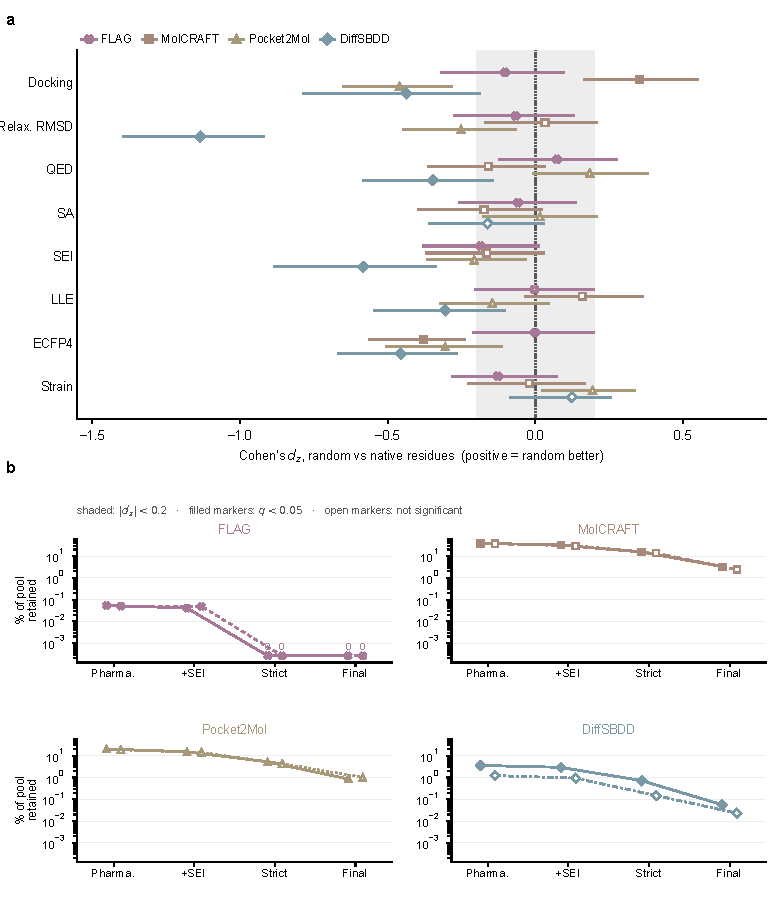
\includegraphics[width=131mm]{figures/si_fig_mapping_control.pdf}
\end{center}

\textbf{a}, Paired effect sizes (Cohen's $d_z$ with 95\% percentile intervals over targets) of the
random-residue arm against the native arm, for the four baselines that accept a residue-type
channel. Filled markers are significant after Benjamini--Hochberg correction across the eight
metrics of that method and open markers are not; the shaded band marks $|d_z|<0.2$. Positive values
mean the random arm scores better. \textbf{b}, Retention through the four-tier screening cascade as
a percentage of each arm's own generated pool, on a logarithmic scale, which makes methods with
different per-target budgets comparable. Solid lines and filled markers are the native arm, dashed
lines and open markers the random arm; a point at the axis floor labelled 0 means that no molecule
of that arm survived the tier. Each method pairs 96--102 DUD-E targets. DiffSBDD, FLAG and
Pocket2Mol were generated for this control at 300 molecules per target with both arms held to
identical per-target pools; MolCRAFT reuses an earlier campaign at about 1000 molecules per target,
whose two arms have unequal pools. GraphBP and ED2Mol take no residue-type input and are not shown.

Panel~\textbf{a} is tabulated in Extended Data Table~9.

\clearpage
\section*{Extended Data Table 1 | NA2smol model configuration}

\begin{center}
\footnotesize
\setlength{\tabcolsep}{6pt}
\begin{tabular}{@{}lc@{}}
\toprule
\textbf{Parameter} & \textbf{Value} \\
\midrule
Hidden dimension & 128 \\
Number of blocks & 1 \\
Number of layers per block & 9 \\
Attention heads & 16 \\
Nearest-neighbour edges ($k$) & 32 \\
Radial basis function (RBF) centres & 20 \\
Time embedding dimension & 1 \\
Time embedding mode & simple \\
Coordinate \(\sigma_1\) & 0.03 \\
Type \(\beta_1\) & 1.5 \\
Discrete steps & 1000 \\
\bottomrule
\end{tabular}
\end{center}

\section*{Extended Data Table 2 | Cross-benchmark scaffold breadth after the screening filter}
Unique canonical SMILES and unique Bemis--Murcko (BM) scaffold counts after the screening filter (docking score $<-8$~kcal~mol$^{-1}$, QED $>0.5$, SA score $<5$, SEI $>0.1$).
\begin{center}\footnotesize
\setlength{\tabcolsep}{3.5pt}
\begin{tabular}{@{}lcccc@{}}
\toprule
 & \multicolumn{2}{c}{\textbf{RNA test set}} & \multicolumn{2}{c}{\textbf{DUD-E}} \\
\cmidrule(lr){2-3}\cmidrule(lr){4-5}
\textbf{Method} & \textbf{Molecules} & \textbf{BM scaffolds} & \textbf{Molecules} & \textbf{BM scaffolds} \\
\midrule
NA2smol    & 6,618 & 5,671 & 32,400 & 24,270 \\
MolCRAFT   &   301 &   287 &  9,012 &  8,316 \\
Pocket2Mol & 1,523 &   700 &  5,039 &  2,714 \\
ED2Mol     &   343 &   274 &  4,262 &  2,795 \\
DiffSBDD   &    31 &    31 &  2,886 &  2,832 \\
FLAG       &     0 &     0 &     55 &     31 \\
GraphBP    &     0 &     0 &      2 &      2 \\
\bottomrule
\end{tabular}\end{center}

NA2smol retains 6,618 molecules spanning 5,671 scaffolds on the RNA test set, approximately 4.3-fold more molecules and 8.1-fold more scaffolds than the best-performing baseline (Pocket2Mol). On DUD-E it retains 32,400 molecules spanning 24,270 scaffolds.

\section*{Extended Data Table 3 | Per-target summary statistics on the RNA test set (27 shared targets)}
Values are mean $\pm$ s.d.\ of per-target medians. The two-sided Wilcoxon $P$ compares NA2smol with its baseline on the shared-target set ($N=27$). Aggregations vary by display: main-text ablation summaries use target-level means; Fig.~3d reports the median of per-target medians; this table reports the mean of per-target medians.
\begin{center}\footnotesize
\setlength{\tabcolsep}{3.5pt}
\begin{tabular}{@{}llccc@{}}
\toprule
\textbf{Category} & \textbf{Metric} & \textbf{NA2smol baseline} & \textbf{NA2smol} & \textbf{$P$} \\
\midrule
\multirow{3}{*}{Drug-likeness}
  & QED                              & $0.475 \pm 0.093$ & $0.622 \pm 0.060$ & $1.5\times10^{-8}$ \\
  & SA score                         & $4.080 \pm 0.863$ & $3.530 \pm 0.537$ & $3.1\times10^{-6}$ \\
  & LLE                              & $3.123 \pm 2.044$ & $4.220 \pm 1.954$ & $5.5\times10^{-3}$ \\
\midrule
\multirow{3}{*}{Docking and geometry}
  & Docking score (kcal mol$^{-1}$)  & $-6.599 \pm 2.432$ & $-7.282 \pm 2.501$ & $1.3\times10^{-4}$ \\
  & SEI                              & $0.103 \pm 0.066$ & $0.103 \pm 0.039$ & 0.35 \\
  & Pose-relaxation RMSD (\AA)       & $1.319 \pm 0.781$ & $1.239 \pm 0.526$ & 1.00 \\
\midrule
Conformational
  & Strain (kcal mol$^{-1}$)         & $730.1 \pm 940.6$ & $351.4 \pm 412.5$ & $1.5\times10^{-8}$ \\
\bottomrule
\end{tabular}\end{center}

NA2smol improves docking score, QED, SA score and LLE, while SEI and pose-relaxation RMSD are statistically indistinguishable. Conformational strain is lower for the full model ($351.4$ versus $730.1$~kcal~mol$^{-1}$).

\section*{Extended Data Table 4 | PoseCheck strain calibration}
Panel A: strain of 37 crystallographic reference ligands of RNA test-set pockets, evaluated from their structurally determined poses using the same smina minimisation and PoseCheck protocol as the generated molecules. All 37 reference ligands are evaluable. Panel B reports uncapped values; Table~1 and Fig.~3d use the censored convention below. ``Strain'' is the PoseCheck local strain energy (kcal~mol$^{-1}$) of the smina-minimised pose. Failures include minimisations exceeding the protocol budget and those with energy $>10^{4}$~kcal~mol$^{-1}$. ``PoseCheck success'' is the percentage of the group for which strain was computed. Reference scale strain is elevated relative to force-field minima; thus, the 200~kcal~mol$^{-1}$ final-tier threshold and cross-configuration differences are interpreted relative to this reference. Panel B: per-molecule strain distributions by configuration. Main-text yield percentages are computed over the full valid-generation pool.

\textbf{Panel A. Crystallographic reference ligands}
\begin{center}\footnotesize
\setlength{\tabcolsep}{5pt}
\begin{tabular}{@{}lccccccc@{}}
\toprule
\textbf{Set} & \textbf{$n$} & \textbf{Success} & \textbf{median} & \textbf{mean} & \textbf{p90} & \textbf{p95} & \textbf{$\le$200, \%} \\
\midrule
Crystal reference ligands & 37 & 37/37 & 48.8 & 147.8 & 272.9 & 746.3 & 81 \\
\bottomrule
\end{tabular}\end{center}

\textbf{Panel B. Generated molecules by configuration}
\begin{center}\scriptsize
\setlength{\tabcolsep}{2.5pt}
\begin{tabular}{@{}lcccccc@{}}
\toprule
\textbf{Set} & \textbf{Eval.\ (pool)} & \textbf{Success} & \textbf{median} & \textbf{p95} & \textbf{$>$10$^{3}$, \%} & \textbf{$>$10$^{4}$, \%} \\
\midrule
NA2smol (full)      & 35,235 (35,358) & 99.7\% & 218.3  & $4.4\times10^{4}$ & 24.0 & 7.7 \\
NA2smol baseline    & 35,959 (36,209) & 99.3\% & 375.6  & $3.0\times10^{4}$ & 26.8 & 8.1 \\
Pretrain Only       & 31,079 (32,782) & 94.8\% & 14,290 & $1.2\times10^{12}$ & 57.6 & 48.5 \\
Pretrain+Constrain  & 35,180 (35,640) & 98.7\% & 284.6  & $1.0\times10^{7}$ & 25.2 & 14.9 \\
\midrule
MolCRAFT            & 34,893 (34,925) & 99.9\% & 125.4  & $3.6\times10^{3}$ & 9.9 & 3.2 \\
ED2Mol              & 29,237 (29,932) & 97.7\% & 22.6   & $1.7\times10^{2}$ & 0.0 & 0.0 \\
\bottomrule
\end{tabular}\end{center}

Median here is computed over all molecules with a finite strain value, so the high-strain tail above $10^{4}$~kcal~mol$^{-1}$ is included. Table~1 instead reports a censored median: values above $10^{4}$~kcal~mol$^{-1}$ and failed evaluations are set to $10^{4}$~kcal~mol$^{-1}$, a median at the bound is reported as $>10^{4}$, and the percentage of successfully evaluated molecules at or below this bound is given in parentheses. Fig.~3d plots per-target medians of the same censored values on the common 27-target set. These summaries therefore differ in aggregation and censoring rather than by discrepancy. The last two columns give the percentage of the full valid-generation pool, including molecules whose evaluation failed or was not completed, above $10^{3}$ and above $10^{4}$~kcal~mol$^{-1}$; the pool is the value in parentheses, and failures are counted in it but never among the exceeding molecules. The main text quotes the $10^{4}$ column, because $10^{4}$~kcal~mol$^{-1}$ is the censoring bound used in Table~1 and Fig.~3d. Success records only that the force-field evaluation finished; it is reported alongside ``Strain evaluated'' in Extended Data Table~8, which additionally requires the energy to stay at or below $10^{4}$~kcal~mol$^{-1}$.
The Pretrain-Only pathology is pervasive: median 14,290~kcal~mol$^{-1}$ with 94.8\% PoseCheck success; 48.5\% of molecules exceed the $10^{4}$~kcal~mol$^{-1}$ bound (41.2\% above $10^{5}$~kcal~mol$^{-1}$; 57.6\% above $10^{3}$~kcal~mol$^{-1}$). ED2Mol shows essentially no strain (median 22.6~kcal~mol$^{-1}$; none above $10^{3}$~kcal~mol$^{-1}$).

\section*{Extended Data Table 5 | Composition of the supervised fine-tuning data}

These are the counts behind the training-set description in the main text; the table records how
the supervised records are distributed, not a result.

{\footnotesize Composition of the supervised fine-tuning data. Counts are curated structures, not the approximately 2.4-million-molecule ligand-only ED pretraining library. Protein structures come from the PDB (experimental) and CrossDocked2020 (docked poses); 2,827 of 48,698 PDB entries were removed because their pockets were too similar to the DUD-E test pockets, using the shape- and ICP-based filter. The 738 nucleic-acid records comprise 457 RNA, 274 DNA and 7 hybrid entries by RCSB polymer annotation (Supplementary Table~4).}

\begin{center}
\small
\begin{tabular}{@{}llc l@{}}
\toprule
\textbf{Training subset} & \textbf{Partition} & \textbf{Records} & \textbf{Target class} \\
\midrule
\multirow{2}{*}{PDB crystal structures}
  & training   & 45,871 & Protein \\
  & validation &  5,000 & Protein \\
CrossDocked2020 docked poses & training & 81,028 & Protein \\
\midrule
\multirow{3}{*}{Nucleic-acid--ligand}
  & total      & 738 & 457 RNA, 274 DNA, 7 hybrid \\
  & training   & 356 & 147 RNA, 202 DNA, 7 hybrid \\
  & validation & 382 & 310 RNA, 72 DNA, 0 hybrid \\
\midrule
\multicolumn{2}{@{}l}{Total, training}   & 127,255 & Protein and nucleic acid \\
\multicolumn{2}{@{}l}{Total, validation} &   5,382 & Protein and nucleic acid \\
\bottomrule
\end{tabular}
\end{center}

\section*{Extended Data Table 6 | Recovery sensitivity to reference overlap}
Recovery is defined by Eqs.~(9)--(10), evaluated on the ECFP4-Tanimoto window $0.25$--$0.50$. Each column re-scores methods on targets surviving the named filter: a target is excluded when all its reference actives reach ECFP4-TS $\geq0.5$ against the fine-tuning training partition (FT) or ligand-only pretraining library (PT). Panel A uses the common seven-method eligible-target set (84 DUD-E; 27 RNA). Targets with no produced molecules score zero recovery and remain in the denominator. $n$ is the number of surviving targets.

\textbf{Panel A. All seven methods on the common eligible-target set}
\begin{center}\footnotesize
\setlength{\tabcolsep}{5pt}
\begin{tabular}{@{}llccc@{}}
\toprule
\textbf{Benchmark} & \textbf{Method} & \textbf{No filter} & \textbf{FT $\geq0.5$} & \textbf{PT $\geq0.5$} \\
\midrule
\multirow{7}{*}{RNA test set ($n=27$ / 18 / 14)}
  & NA2smol    & \textbf{0.218} & \textbf{0.250} & 0.053 \\
  & ED2Mol     & 0.077 & 0.106 & \textbf{0.085} \\
  & Pocket2Mol & 0.080 & 0.098 & 0.011 \\
  & MolCRAFT   & 0.059 & 0.026 & 0.039 \\
  & DiffSBDD   & 0.042 & 0.036 & 0.044 \\
  & FLAG       & 0.002 & 0.000 & 0.004 \\
  & GraphBP    & 0.004 & 0.000 & 0.000 \\
\midrule
\multirow{7}{*}{DUD-E ($n=84$ / 84 / 81)}
  & NA2smol    & \textbf{0.692} & \textbf{0.578} & 0.238 \\
  & DiffSBDD   & 0.447 & 0.447 & \textbf{0.455} \\
  & ED2Mol     & 0.514 & 0.436 & 0.171 \\
  & Pocket2Mol & 0.502 & 0.361 & 0.169 \\
  & MolCRAFT   & 0.345 & 0.273 & 0.067 \\
  & FLAG       & 0.122 & 0.122 & 0.121 \\
  & GraphBP    & 0.072 & 0.072 & 0.074 \\
\bottomrule
\end{tabular}\end{center}

Excluding targets whose actives resemble the fine-tuning partition leaves NA2smol ahead (0.250 against 0.106 on RNA; 0.578 against 0.436 on DUD-E). Excluding targets whose actives resemble the pretraining library changes the order: NA2smol falls to 0.053 on RNA (ED2Mol: 0.085) and 0.238 on DUD-E (DiffSBDD: 0.455). Because that filter removes targets whose chemistry the pretraining stage covers, a drop is expected.

\textbf{Panel B. RNA test-set training configurations}
\begin{center}\footnotesize
\setlength{\tabcolsep}{5pt}
\begin{tabular}{@{}lccc@{}}
\toprule
\textbf{Configuration} & \textbf{No filter} & \textbf{FT $\geq0.5$} & \textbf{PT $\geq0.5$} \\
\midrule
Full NA2smol            & \textbf{0.218} & \textbf{0.250} & 0.053 \\
Pretrain+Constrain      & 0.132 & --- & --- \\
Pretrain Only           & 0.035 & --- & --- \\
No-pretraining baseline & 0.141 & --- & --- \\
\bottomrule
\end{tabular}\end{center}

\section*{Extended Data Table 7 | Sensitivity of RNA test-set recovery to chemically similar reference actives}
Recovery is defined by Eqs.~(9)--(10) (ECFP4-Tanimoto window $0.25$--$0.50$). Analogue filters remove reference actives with max ECFP4-Tanimoto similarity $\geq0.5$ to the fine-tuning training partition (FT) or ligand-only pretraining library (PT). Each change compares filtered and original references on the identical eligible-target subset. The full model shows the largest reduction under the PT filter ($-0.198$; Pretrain+Constrain: $-0.099$; Pretrain Only: $-0.014$). Filtering removes reference actives only and does not affect the generated molecules.

\begin{center}\footnotesize
\setlength{\tabcolsep}{5pt}
\begin{tabular}{@{}lccc@{}}
\toprule
 & Unfiltered & \multicolumn{2}{c}{Change after analogue removal} \\
\cmidrule(lr){3-4}
Model configuration & Recovery (27 targets) & FT (18 targets) & PT (14 targets) \\
\midrule
No-pretraining baseline & 0.141 & $-0.077$ & --- \\
Pretrain Only & 0.034 & $-0.017$ & $-0.014$ \\
Pretrain+Constrain & 0.132 & $-0.016$ & $-0.099$ \\
\textbf{Full NA2smol} & \textbf{0.218} & $-0.077$ & $-0.198$ \\
\bottomrule
\end{tabular}
\end{center}

\section*{Extended Data Table 8 | Normalised scores behind the panels of Figs.~2 and 3}
Values underlying Figs.~2a, 2d and 3a. Fig.~3a displays the scores as a radar chart, in which each axis plots the normalised score $s_m$ at radial coordinate $r_m = 1 + 2s_m$; raw metric medians are in Table~1 and the normalised scores are given below. In Table~1, property values are pooled medians over all of a method's molecules, the same molecule pool used by the retention-curve integrals. Here, the metric axes for docking, RMSD, QED, SA, SEI and strain are the normalised integrals of their respective retention curves ($\log_{10}$ scale for strain). In Table~1, Strain is the median over all molecules after values above $10^{4}$~kcal~mol$^{-1}$ and evaluations that did not finish are set to $10^{4}$~kcal~mol$^{-1}$; when this median reaches the bound it is reported as $>10^{4}$, and the percentage of molecules successfully evaluated at or below the bound is given in parentheses, so this column describes both screening-stable molecules and the failure burden. The uncapped distribution, including the high-strain tail, is in Extended Data Table~4, whereas Fig.~3d shows the median of per-target medians computed from the same censored values; the three summaries therefore differ in aggregation and censoring. Raw Dock.\ and Strain values are in kcal~mol$^{-1}$ (scientific notation above $10^3$) and RMSD is in \AA. ECFP4 is the observed recovery defined by Eqs.~(9)--(10). The ECFP4 axis uses that raw recovery directly without rescaling: recovery is already the area under the per-target retention curve and lies in $[0,1]$, so no cross-method normalisation is needed. The first table below gives the seven normalised scores $s_m$, and the second gives strain coverage: the percentage of each method's molecule pool whose strain could be computed within the budget and stayed at or below $10^{4}$~kcal~mol$^{-1}$. Failures are retained in the denominator $n$ of pass rates. NA2smol appears under both Fig.~2d and Fig.~3a because the full model represents the same output set in both panels.

\bigskip

\noindent\begin{minipage}{\textwidth}
\textbf{Normalised scores $s_m$}
\begin{center}\footnotesize
\setlength{\tabcolsep}{3.5pt}
\begin{tabular}{@{}llccccccc@{}}
\toprule
\textbf{Method} & \textbf{$n$} & \textbf{QED} & \textbf{Strain} & \textbf{SA} & \textbf{RMSD} & \textbf{Dock.} & \textbf{ECFP4} & \textbf{SEI} \\
\midrule
\multicolumn{9}{@{}l}{\textit{Fig. 2a — DUD-E protein}} \\
NA2smol & 104,980 & 0.627 & 0.678 & 0.627 & 0.658 & 0.641 & 0.656 & 0.444 \\
MolCRAFT & 98,257 & 0.523 & 0.604 & 0.484 & 0.827 & 0.801 & 0.331 & 0.416 \\
Pocket2Mol & 65,662 & 0.559 & 0.653 & 0.658 & 0.468 & 0.386 & 0.417 & 0.375 \\
ED2Mol & 93,293 & 0.736 & 0.862 & 0.517 & 0.375 & 0.389 & 0.482 & 0.495 \\
DiffSBDD & 102,000 & 0.491 & 0.480 & 0.236 & 0.179 & 0.311 & 0.457 & 0.211 \\
GraphBP & 73,598 & 0.467 & 0.122 & 0.151 & 0.035 & 0.048 & 0.093 & 0.158 \\
FLAG & 83,093 & 0.418 & 0.745 & 0.139 & 0.115 & 0.136 & 0.142 & 0.156 \\
\midrule
\multicolumn{9}{@{}l}{\textit{Fig. 2d — RNA test set}} \\
NA2smol & 35,358 & 0.617 & 0.616 & 0.572 & 0.546 & 0.512 & 0.218 & 0.392 \\
MolCRAFT & 34,925 & 0.434 & 0.695 & 0.534 & 0.827 & 0.503 & 0.059 & 0.229 \\
Pocket2Mol & 34,097 & 0.540 & 0.451 & 0.657 & 0.486 & 0.377 & 0.080 & 0.273 \\
ED2Mol & 29,932 & 0.700 & 0.871 & 0.564 & 0.441 & 0.272 & 0.077 & 0.448 \\
DiffSBDD & 36,999 & 0.464 & 0.698 & 0.258 & 0.070 & 0.116 & 0.080 & 0.131 \\
GraphBP & 20,571 & 0.451 & 0.153 & 0.145 & 0.042 & 0.053 & 0.004 & 0.202 \\
FLAG & 27,195 & 0.385 & 0.839 & 0.137 & 0.137 & 0.103 & 0.015 & 0.151 \\
\midrule
\multicolumn{9}{@{}l}{\textit{Fig. 3a — RNA test set, four configurations}} \\
Baseline & 36,209 & 0.494 & 0.560 & 0.507 & 0.532 & 0.406 & 0.141 & 0.345 \\
Pretrain Only & 32,782 & 0.501 & 0.286 & 0.319 & 0.504 & 0.536 & 0.035 & 0.380 \\
Pretrain+Constrain & 35,640 & 0.597 & 0.549 & 0.443 & 0.514 & 0.523 & 0.132 & 0.403 \\
NA2smol & 35,358 & 0.617 & 0.616 & 0.572 & 0.546 & 0.512 & 0.218 & 0.392 \\
\bottomrule
\end{tabular}
\end{center}
\end{minipage}

\bigskip

\noindent\begin{minipage}{\textwidth}
\textbf{Strain coverage (percent of each method molecule pool)}
\begin{center}\footnotesize
\setlength{\tabcolsep}{3.5pt}
\begin{tabular}{@{}llccc@{}}
\toprule
\textbf{Method} & \textbf{$n$} & \textbf{Strain evaluated} & \textbf{pass@500} & \textbf{pass@200} \\
\midrule
\multicolumn{5}{@{}l}{\textit{Fig. 2a — DUD-E protein}} \\
NA2smol & 104,980 & 95.1\% & 78.7\% & 63.9\% \\
MolCRAFT & 98,257 & 93.1\% & 71.1\% & 39.1\% \\
Pocket2Mol & 65,662 & 97.4\% & 86.2\% & 45.7\% \\
ED2Mol & 93,293 & 97.2\% & 97.1\% & 93.6\% \\
DiffSBDD & 102,000 & 81.8\% & 55.6\% & 42.6\% \\
GraphBP & 73,598 & 29.5\% & 11.6\% & 8.2\% \\
FLAG & 83,093 & 95.5\% & 84.2\% & 76.7\% \\
\midrule
\multicolumn{5}{@{}l}{\textit{Fig. 2d — RNA test set}} \\
NA2smol & 35,358 & 92.0\% & 66.6\% & 47.7\% \\
MolCRAFT & 34,925 & 96.7\% & 84.5\% & 66.4\% \\
Pocket2Mol & 34,097 & 70.5\% & 58.9\% & 22.9\% \\
ED2Mol & 29,932 & 97.7\% & 97.6\% & 94.8\% \\
DiffSBDD & 36,999 & 93.9\% & 79.5\% & 70.0\% \\
GraphBP & 20,571 & 35.3\% & 14.9\% & 10.7\% \\
FLAG & 27,195 & 95.1\% & 90.1\% & 86.7\% \\
\midrule
\multicolumn{5}{@{}l}{\textit{Fig. 3a — RNA test set, four configurations}} \\
Baseline & 36,209 & 91.2\% & 58.1\% & 29.2\% \\
Pretrain Only & 32,782 & 46.3\% & 30.2\% & 13.2\% \\
Pretrain+Constrain & 35,640 & 83.8\% & 64.4\% & 37.0\% \\
NA2smol & 35,358 & 92.0\% & 66.6\% & 47.7\% \\
\bottomrule
\end{tabular}
\end{center}
\end{minipage}
\noindent{\footnotesize Strain evaluated counts a molecule as failed when the force-field evaluation did not finish inside the budget \emph{or} its strain exceeded $10^{4}$~kcal~mol$^{-1}$; failures stay in the denominator $n$. This is a stricter quantity than the PoseCheck success fraction of Extended Data Table~4, which records only whether the evaluation finished. pass@500 and pass@200 are percentages of the whole pool, not of the evaluated subset.}\par

\section*{Extended Data Table 9 | Sensitivity of each baseline to randomised residue assignment}

Protein-oriented structure-based generators cannot encode nucleotide residues, so the RNA test set was scored with every nucleic-acid residue reassigned to one of the 20 amino-acid types before inference (Methods). To test whether that reassignment is itself responsible for the ordering seen on the benchmark, each baseline that accepts a residue-type channel was run on DUD-E twice: once with its native protein residue types, and once with every residue type reassigned at random while atomic coordinates, atom names and all sampling settings were held fixed. DiffSBDD, FLAG and Pocket2Mol were run for this control, and MolCRAFT was run earlier on the same protocol; GraphBP and ED2Mol take no residue-type input (element-only and electron-density conditioning, respectively), so the control has no meaning for them. Both arms of every pair were scored with the identical docking, screening and recovery pipeline, and the scrambling rule is the deterministic hash described in Methods.

Both arms of a pair were trimmed to the same number of molecules at every target, so every median and every retention count below rests on identical pools; DiffSBDD, FLAG and Pocket2Mol were generated for this control at 300 molecules per target and MolCRAFT reuses its earlier campaign at about 1000. The budget is not cosmetic: at a budget of 25 molecules per target, Pocket2Mol showed no metric beyond $|d_z|=0.24$ and would have been called insensitive, whereas at 300 its docking score, pose-relaxation RMSD and ECFP4 similarity are all significantly degraded. Small controls therefore understate sensitivity, and the three regenerated methods use the same budget so their effect sizes are directly comparable. MolCRAFT is the exception in Panel~B only: its two arms were generated in an earlier campaign with different yields (76,351 native and 98,257 random molecules over the same 100 targets), so its per-target medians remain paired but its retention counts rest on unequal pools.
\begin{samepage}
\textbf{Panel A. Paired metric effects}
\begin{center}\scriptsize
\setlength{\tabcolsep}{2pt}
\begin{tabular}{@{}llcccccc@{}}
\toprule
\textbf{Method} & \textbf{Metric} & \textbf{$n$ targets} & \textbf{Native} & \textbf{Random} & \textbf{$\Delta$} & \textbf{$d_z$ (95\% CI)} & \textbf{$q$} \\
\midrule
\textit{MolCRAFT} & Docking & 100 & $-9.86$ & $-10.05$ & 0.17 & 0.35 (0.16, 0.55) & 0.007 \\
 & RMSD & 100 & 0.371 & 0.371 & 0.005 & 0.03 ($-0.17$, 0.21) & 0.861 \\
 & QED & 100 & 0.564 & 0.561 & $-0.012$ & $-0.16$ ($-0.36$, 0.03) & 0.158 \\
 & SA & 100 & 4.08 & 4.10 & $-0.07$ & $-0.17$ ($-0.40$, 0.02) & 0.086 \\
 & SEI & 100 & 0.115 & 0.108 & $-0.004$ & $-0.16$ ($-0.37$, 0.03) & 0.189 \\
 & LLE & 100 & 7.07 & 7.27 & 0.17 & 0.16 ($-0.04$, 0.36) & 0.150 \\
 & ECFP4 & 100 & 0.181 & 0.176 & $-0.007$ & $-0.38$ ($-0.56$, $-0.24$) & $<10^{-3}$ \\
 & Strain & 100 & 254 & 264 & $-1$ & $-0.02$ ($-0.23$, 0.17) & 0.398 \\
\midrule
\textit{Pocket2Mol} & Docking & 102 & $-8.67$ & $-8.38$ & $-0.30$ & $-0.46$ ($-0.65$, $-0.28$) & $<10^{-3}$ \\
 & RMSD & 102 & 0.829 & 0.856 & $-0.050$ & $-0.25$ ($-0.45$, $-0.06$) & 0.039 \\
 & QED & 102 & 0.542 & 0.556 & 0.016 & 0.18 ($-0.01$, 0.38) & 0.183 \\
 & SA & 102 & 4.58 & 4.58 & 0.01 & 0.01 ($-0.18$, 0.21) & 0.695 \\
 & SEI & 102 & 0.097 & 0.092 & $-0.007$ & $-0.21$ ($-0.37$, $-0.03$) & 0.239 \\
 & LLE & 102 & 5.58 & 5.45 & $-0.17$ & $-0.15$ ($-0.33$, 0.05) & 0.225 \\
 & ECFP4 & 99 & 0.174 & 0.174 & $-0.004$ & $-0.30$ ($-0.51$, $-0.11$) & 0.022 \\
 & Strain & 102 & 33 & 31 & 7 & 0.19 (0.02, 0.34) & 0.489 \\
\midrule
\textit{DiffSBDD} & Docking & 102 & $-5.51$ & $-4.76$ & $-1.01$ & $-0.44$ ($-0.79$, $-0.18$) & $<10^{-3}$ \\
 & RMSD & 102 & 2.833 & 3.343 & $-0.548$ & $-1.13$ ($-1.40$, $-0.92$) & $<10^{-3}$ \\
 & QED & 102 & 0.486 & 0.467 & $-0.031$ & $-0.35$ ($-0.58$, $-0.14$) & $<10^{-3}$ \\
 & SA & 102 & 5.63 & 5.71 & $-0.08$ & $-0.16$ ($-0.36$, 0.03) & 0.116 \\
 & SEI & 102 & 0.058 & 0.045 & $-0.016$ & $-0.58$ ($-0.88$, $-0.34$) & $<10^{-3}$ \\
 & LLE & 102 & 3.11 & 2.91 & $-0.76$ & $-0.31$ ($-0.55$, $-0.10$) & $<10^{-3}$ \\
 & ECFP4 & 99 & 0.155 & 0.151 & $-0.005$ & $-0.46$ ($-0.67$, $-0.26$) & $<10^{-3}$ \\
 & Strain & 102 & 185 & 192 & 20 & 0.12 ($-0.09$, 0.26) & 0.499 \\
\midrule
\textit{FLAG} & Docking & 96 & $-3.91$ & $-3.84$ & $-0.04$ & $-0.10$ ($-0.32$, 0.10) & 0.394 \\
 & RMSD & 96 & 3.215 & 3.252 & $-0.020$ & $-0.07$ ($-0.28$, 0.13) & 0.450 \\
 & QED & 96 & 0.405 & 0.405 & 0.003 & 0.07 ($-0.12$, 0.28) & 0.498 \\
 & SA & 96 & 6.52 & 6.62 & $-0.02$ & $-0.06$ ($-0.26$, 0.14) & 0.713 \\
 & SEI & 96 & 0.043 & 0.042 & $-0.001$ & $-0.19$ ($-0.38$, 0.01) & 0.394 \\
 & LLE & 96 & 4.76 & 4.91 & $-0.00$ & $-0.00$ ($-0.21$, 0.20) & 0.881 \\
 & ECFP4 & 93 & 0.120 & 0.119 & $-0.000$ & $-0.00$ ($-0.21$, 0.20) & 0.779 \\
 & Strain & 96 & 26 & 29 & $-3$ & $-0.13$ ($-0.28$, 0.07) & 0.394 \\
\midrule
\bottomrule
\end{tabular}\end{center}

Oriented $\Delta$ is the mean paired difference in the direction of better performance (positive means the random arm scores better); $d_z$ is Cohen's $d$ for paired samples with a 95\% percentile interval over targets, and $q$ is the Wilcoxon signed-rank $P$ value after Benjamini--Hochberg correction across the eight metrics of that method.

\end{samepage}
\begin{samepage}
\textbf{Panel B. Screening retention under the four-tier cascade}
\begin{center}\scriptsize
\setlength{\tabcolsep}{4pt}
\begin{tabular}{@{}llrrrrr@{}}
\toprule
\textbf{Method} & \textbf{Arm} & \textbf{All} & \textbf{Pharma.} & \textbf{+SEI} & \textbf{Strict} & \textbf{Final tier} \\
\midrule
\textit{MolCRAFT} & Native & 76,351 & 29,639 & 24,377 & 11,667 & 2,471 \\
\textit{MolCRAFT} & Random & 98,257 & 36,410 & 28,938 & 13,287 & 2,361 \\
\midrule
\textit{Pocket2Mol} & Native & 30,515 & 6,197 & 4,607 & 1,580 & 260 \\
\textit{Pocket2Mol} & Random & 30,515 & 5,760 & 4,252 & 1,306 & 306 \\
\midrule
\textit{DiffSBDD} & Native & 30,600 & 1,093 & 884 & 217 & 17 \\
\textit{DiffSBDD} & Random & 30,600 & 373 & 285 & 45 & 7 \\
\midrule
\textit{FLAG} & Native & 24,437 & 13 & 10 & 0 & 0 \\
\textit{FLAG} & Random & 24,437 & 12 & 12 & 0 & 0 \\
\midrule
\bottomrule
\end{tabular}\end{center}

\end{samepage}
Counts are valid generated molecules surviving each successive tier of the manuscript cascade (Pharma.: docking $<-8$~kcal~mol$^{-1}$, QED $>0.5$, SA $<5$; +SEI adds SEI $>0.1$; Strict: docking $<-9$~kcal~mol$^{-1}$, QED $>0.5$, SA $<5$, SEI $>0.15$; Final tier adds QED $>0.6$, SA $<4$, SEI $>0.2$ and strain $<200$~kcal~mol$^{-1}$). Both arms of a pair were generated and scored with the same settings, so the two rows are directly comparable within a method.

\noindent\textbf{Summary.} 
MolCRAFT: 2 of 8 metrics at $q<0.05$ (Docking score, ECFP4), largest shift ECFP4 ($|d_z|=0.38$); Pocket2Mol: 3 of 8 metrics at $q<0.05$ (Docking score, Relax. RMSD, ECFP4), largest shift Docking score ($|d_z|=0.46$); DiffSBDD: 6 of 8 metrics at $q<0.05$ (Docking score, Relax. RMSD, QED, SEI, LLE, ECFP4), largest shift Relax. RMSD ($|d_z|=1.13$); FLAG: none of 8 metrics at $q<0.05$, largest shift SEI ($|d_z|=0.19$). 
Randomising residue identity therefore does not act uniformly across the four baselines; the effect scales with how much of the pocket chemistry each encoder carries in its residue channel. FLAG is unaffected on every metric. MolCRAFT and Pocket2Mol sit in between and disagree with themselves across axes: MolCRAFT docks slightly better from scrambled pockets while its best ECFP4 similarity falls, and Pocket2Mol loses docking quality, pose relaxation and ECFP4 similarity while gaining on the property axes. DiffSBDD is the extreme case, because its C$\alpha$-level representation encodes the pocket almost entirely through the amino-acid one-hot channel, so scrambling removes the signal it conditions on and degrades six of eight metrics, with retention at the first screening tier falling from 1,093 to 373 molecules on the same target set. Two consequences follow for how the external comparison should be read. Random residue assignment does not manufacture the benchmark ordering for FLAG, and only mildly perturbs MolCRAFT and Pocket2Mol, so those comparisons stand as performance context. For DiffSBDD the mapping is not a neutral compatibility device, and its RNA results should be read as a lower bound obtained under a degraded pocket representation rather than as an estimate of that architecture's ceiling.

\end{document}
